% ============================================================
% Combined AUC Heatmap Figure (Fig. 3 + Fig. 4 merged)
% ============================================================
%
% Option 1: Using subcaption package (recommended for LaTeX)
% Add to your preamble: \usepackage{subcaption}
%
% --- Subfigure approach (two separate images) ---

\begin{figure}[htbp]
  \centering
  \begin{subfigure}[t]{0.48\textwidth}
    \centering
    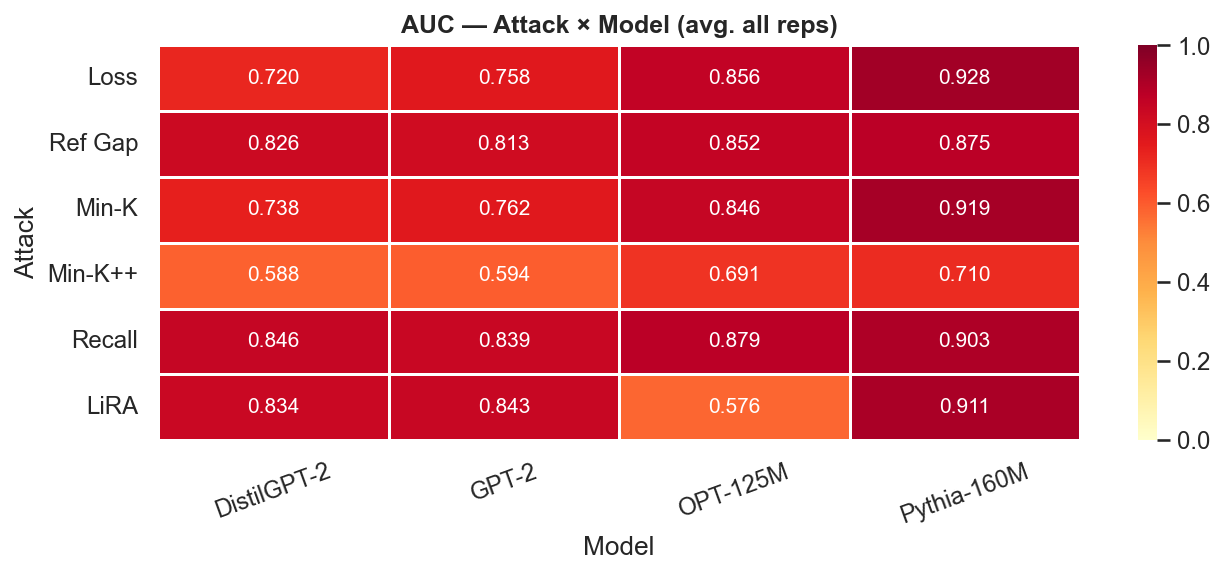
\includegraphics[width=\textwidth]{figures/fig_02.png}
    \caption{AUC heatmap across attacks and models.}
    \label{fig:auc-model}
  \end{subfigure}
  \hfill
  \begin{subfigure}[t]{0.48\textwidth}
    \centering
    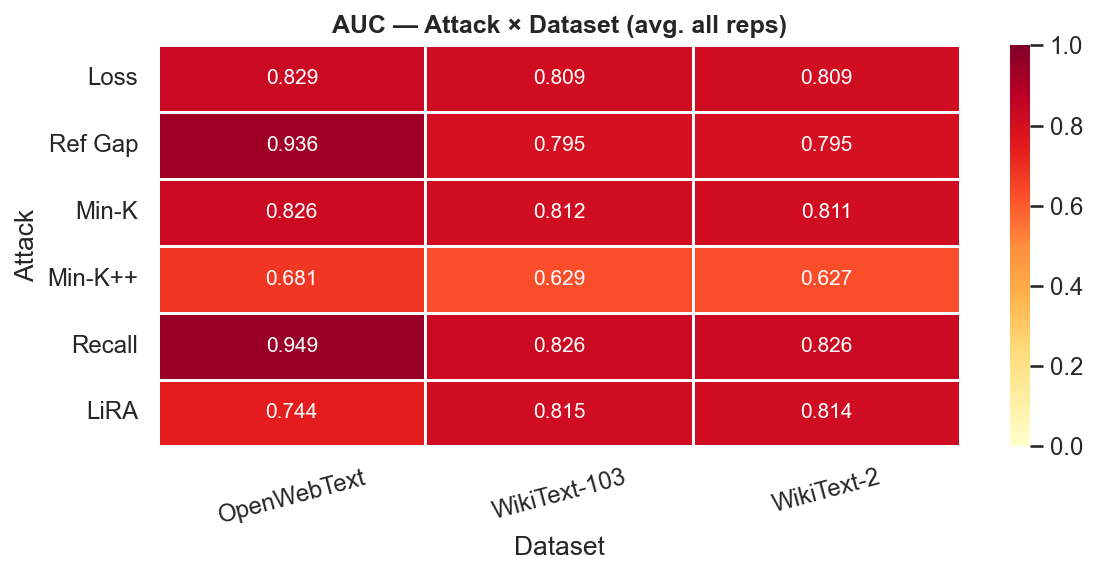
\includegraphics[width=\textwidth]{figures/fig_03.png}
    \caption{AUC heatmap across attacks and datasets.}
    \label{fig:auc-dataset}
  \end{subfigure}
  \caption{AUC heatmaps averaged over all repetitions.
    (a)~Pythia-160M exhibits the highest vulnerability; OPT-125M shows anomalous LiRA performance.
    (b)~OpenWebText yields higher AUC for reference-based attacks; WikiText variants produce near-identical results.}
  \label{fig:auc-heatmaps}
\end{figure}

% ============================================================
%
% Option 2: Single combined image (no subcaption needed)
% Use this if you prefer a single pre-composed image.
%
% \begin{figure}[htbp]
%   \centering
%   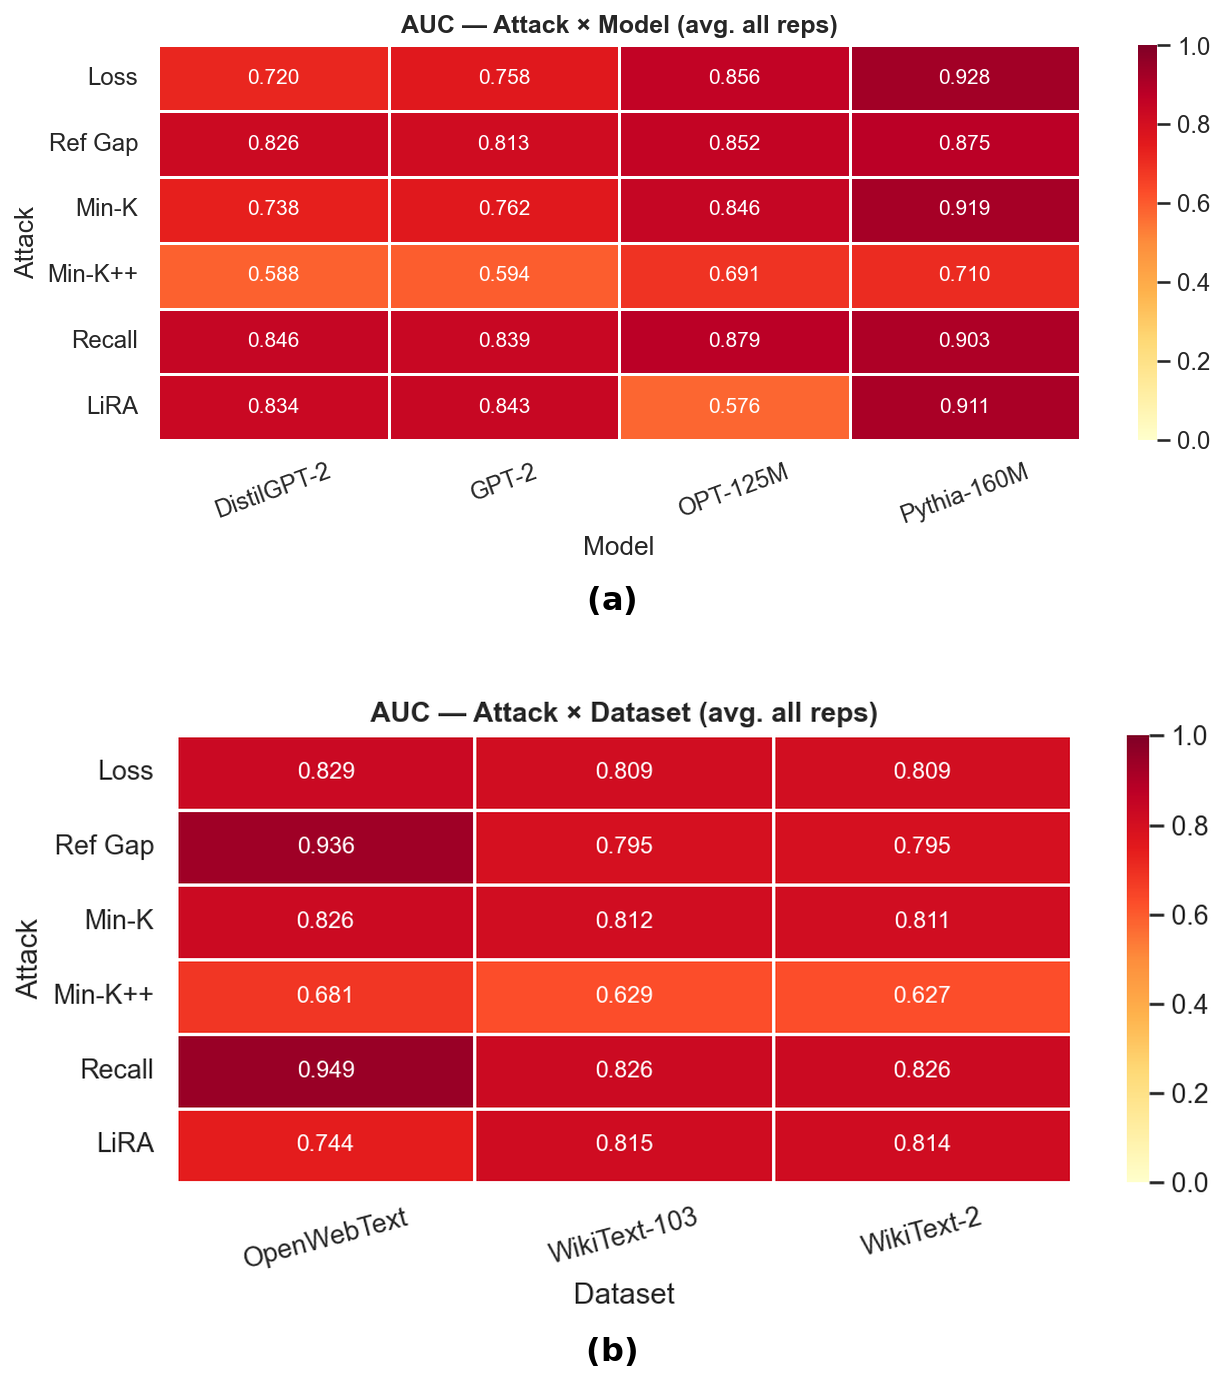
\includegraphics[width=\textwidth]{figures/fig_combined_auc_heatmaps_labeled.png}
%   \caption{AUC heatmaps averaged over all repetitions.
%     (a)~Attack $\times$ Model: Pythia-160M exhibits the highest vulnerability;
%     OPT-125M shows anomalous LiRA performance.
%     (b)~Attack $\times$ Dataset: OpenWebText yields higher AUC for
%     reference-based attacks; WikiText variants produce near-identical results.}
%   \label{fig:auc-heatmaps}
% \end{figure}
